\documentclass[iop,revtex4]{emulateapj}
\usepackage{natbib}
\usepackage{amsfonts}
\usepackage{amssymb}
\usepackage[printonlyused]{acronym}
\usepackage{amsmath,amsthm}
\usepackage{enumerate}
\usepackage{amsmath, amssymb, mathrsfs}
\usepackage{rotate}
\usepackage{lscape}
\shorttitle{3D Simulations of Accretion Torus}
%\shortauthors{Jacobson \& Frebel}
\begin{document}
\newacro{MHD}[MHD]{Magnetohydrodynamics}
\acrodef{MHD}[MHD]{Magnetohydrodynamics}
\newacro{PPI}[PPI]{Papaloizou-Pringle Instability}
\acrodef{PPI}[PPI]{Papaloizou-Pringle Instability}
%\acrodef{MRI}[MRI]{Magnetorotational Instability}
\newacro{MRI}[MRI]{magnetorotational instability}
\acrodef{MRI}[MRI]{magnetorotational instability}
\newacro{SMR}[smr]{Static Mesh Refinement}
\acrodef{SMR}[smr]{Static Mesh Refinement}
\newacro{FFT}[FFT]{Fast Fourier Transform}
\acrodef{FFT}[FFT]{Fast Fourier Transform}
\newacro{CFL}[CFL]{Courant Friedrichs Lewy}
\acrodef{CFL}[CFL]{Courant Friedrichs Lewy}
\newcommand{\app}{\textit{ Athena++ }}
\title{Three-dimensional simulations of instabilities in accretion disk torus}
\author{Jung Lin (Doris) Lee}
 \begin{abstract}
Accretion disks can be found in a variety of astrophysical systems, such as around young stars and black holes. It has been long proposed that fluid instabilities can generate the turbulent viscosity required for driving outward angular momentum transport in accretion flows. In this project, we investigate the dynamics of an accretion disk torus using the new \acf{MHD} code, \app . First, we examine the hydrodynamical behavior of the torus when perturbed by small non-axisymmetric modes and show that it gives rise to a global fluid instability known as the \acf{PPI}. We numerically simulate a slender torus and track its evolution into non-linear regimes. We experiment with various physical and numerical parameters to explore how it affects the torus simulation. By computing the mode amplitude in the linear regime before saturation, we can quantify the mode growth and compare the results with the predicted analytical mode growth. Then, we investigate the behavior of a torus initialized with a weak toroidal magnetic field and examine the effects of \acf{MRI}. Using high-resolution simulations, we are able to resolve the higher order modes of the \ac{MRI}. We computed the mass accretion history of the instabilities and found that \ac{MRI} is significantly more effective in transporting the angular momentum outward than compared to \ac{PPI}. Convergence with previous results in literature demonstrates the robustness of \app  in handling both types of instabilities in accretion disk tori. 
\end{abstract}
\keywords{instabilities, hydrodynamics, methods:numerical, accretion:accretion disks}%,\ac{MHD}}
\section{Introduction}\label{sec:intro}
\par Accretion disk physics are important in various astrophysical systems, such as circumstellar disks around young stars.  If angular momentum are conserved in these systems, it is necessary for the angular momentum to transport outward in order for material from the disc to accrete onto the central object. One of the central questions in accretion disc physics is what are possible mechanisms that enable outward angular momentum transport in discs. Observational evidence of high-energy jets and outflows are signatures of such transport. On the theoretical front, most of the efforts have been directed towards the development of better numerical scheme and codes to realistically simulate such systems. 
\par In this project, we use the new hydrodynamic, \ac{MHD} code, \app, to study two types of fluid instabilities in accretion disk tori. The first is the \ac{PPI}, a type of global, hydrodynamical instability that occurs in accretion tori with constant angular momentum throughout. The second instability we examined is the \ac{MRI}, which is a local, \ac{MHD} instability that has gained considerable recent interest due to its effectiveness in providing outward angular momentum transport in the disc.
\par In Section 1%~\ref{ppi}
, I will describe how we initialize the \ac{PPI} simulation and the numerical methods that we use to simulate these systems. Section 2%~\ref{mri} 
details the basics setup for our \ac{MRI} study and explore the effects of changing the grid resolutions. Finally, Section 3%~\ref{comparison} 
highlights the nature of these instabilities by comparing their mode growth and mass accretion rate history which tells us how effective the instabilities can transport angular momentum outwards.
\section{Papaloizou Pringle Instability\label{ppi}}
An accretion tori can be realized in accretion disk near its Eddginton luminosity, where the torus is in hydrostatic equilibrium between radiation pressure and inward gravitational force. In high accretion rate or high energy systems, such as AGNs and qusars, radiation near the poles creates a hollow region near the central accreting object and results in the toroidal geometry. In scenarioes of discs with very high internal temperature, the pressure gradient can get so large that the rotational profile deviate significantly from a Keplerian disk.  In  \cite{Papaloizou:1984A}, the authors consider a torus with a rotational velocity profile that sets up a constant angular momentum. By conducting a linear stability analysis, they found that non-axisymmetric perturbations result in exponential mode growth on the order of dynamical timescale, resulting in the global, hydrodynamical instability known as the \acf{PPI}. \footnote{The more general case of a non-uniform angular momentum torus is studied in \cite{Papaloizou:1985A} which additionally give rise to Kelvin-Helmholtz-like instabilities.} Further studies conducts linear stability analysis of the case of the slender torus using a set of 2D height-averaged equations. These are applicable when examining lower order modes on the principal branch where the scaled azimuthal wavenumber $\beta<0.59$, since the torus is in vertical hydrostatic equilibrium. 
\par However, linear stability analysis breaks down after Papaloizou-Pringle instability arises and the system becomes nonlinear. Three-dimensional numerical simulation is required to track the evolution of the torus in this nonlinear regime. \cite{Hawley:1990A} found that the instability breaks the torus up into independent ``planets" , which is a more stable configuration than the instabilities in the torus. Before the discovery of \ac{MRI} (\cite{Balbus:1991A}), \ac{PPI} provided a possible mechanism to generate turbulent viscosity for angular momentum transport in disks. 
\par Even though the \ac{PPI} was originally proposed as a possible mechanism for generating the turbulent viscosity required for outward angular momentum transport, it is not as effective as the \ac{MRI} and requires an idealized initial setup for the instability to occur that is unlikely to realize astrohphysical settings. We treat the Papaloizou-Pringle instability as test case for academic interest since there exist an analytical prediction for the mode growth \cite{Goldreich:1986A} which serves as a benchmark with which we could compare the results of numerical simulation. As noted in \cite{Hawley:1991A}, numerical diffusion tends to suppress mode growth and stabilizes the torus. Therefore, this serves as a useful test case for the hydrodynamics scheme in \app. In this project, we reproduce the Hawley's 3D finite difference simulation with a higher grid resolution and using more accurate hydrodynamics schemes in the new \app code.
\subsection{Numerical Methods}
To observe the effects of how the instability is affected by different parameters, we first conducted a series of low resolution $64^3$ numerical experiments to qualitatively examine the behavior of the m=1 mode. In order to track its evolution, the simulations are carried out far into the nonlinear regime until the pressure maximum spiral into the innermost boundary. The results are summarized in Table~\ref{parameters}. $R_0/R_B$, the ratio between the radius to pressure max and to inner boundary, defines the radial dynamic range of the grid.  All the models uses an adiabatic equation of state where $\gamma$=5/3. $t_{run}$ is denoted in units of orbits. The computation is carried out on Hopper, NERSC's Cray XE6 System and Edison, a Cray XC30 System.
\subsubsection{Initial Conditions\label{sec:IC}}
\par As derived in \cite{Papaloizou:1984A}, the initial conditions of the torus satisfies hydrostatic equilibrium.
\begin{equation}
-\frac{\nabla P}{\rho}-\nabla \psi_{pm} +\Omega^2\tilde{\omega}\mathbf{\hat{\tilde{\omega}}}=0
\end{equation}
where $\psi_{pm}$ is the pseudo-Newtonian potential used in \cite{Blaes:1987A}
\begin{equation}
\phi = \frac{-GM}{r-R_G}
\end{equation}
 Here we approximate the Schwarzschild radius $R_G=0$ since $R_G <<R_0$ of the torus. The torus density that satisfies this condition is given by: 
\begin{equation}
\rho(r,\theta) = \Bigg[\frac{GM}{(n+1)AR_0}\Big[\frac{R_0}{r}-\frac{1}{2}\Bigg(\frac{R_0}{r sin\theta}\Bigg)^2-\frac{1}{2d}\Big]\Bigg]^n
\end{equation}
The cells in each r-$\theta$ slice of a torus is divided into a more refined 10$\times$10 subgrid to better enforce the equilibrium condition in the initial condition. We ensured the stability of the torus by evolving it for over 30 orbits without perturbation and showed that there is no unstable modes. 
\par The torus pressure is computed directly from the torus density, as given by the polytrope equation $P = A\rho^\gamma$.  The constant A can be computed by setting $\rho_{max}$ = 1, and therefore $$A =\frac{(d-1)}{2d(n+1)}.$$
The gas density outside the torus ($d_0$) is chosen to be $10^{-4}$ and an ambient pressure profile of P=$d_0$/r is setup in the initial condition. At the boundary of the torus, we compute the torus density compare it with $d_0$ and take the larger of the two to be the density. This smoothed out the discontinuities due to the piecewise definition of the physical quantities at the boundary of the torus, as shown in the radial profile in Fig.~\ref{d_p_profile} .
\begin{figure}
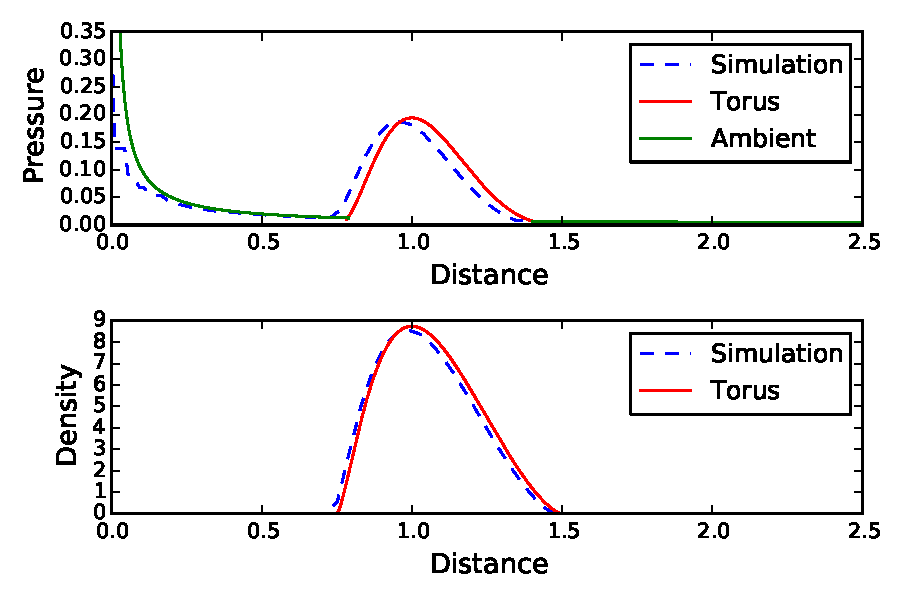
\includegraphics[width=0.45\textwidth]{plots/profile.pdf}
\caption{Density and Pressure profile in the initial condition taken from a $\theta = \pi/2$ slice.}
\label{d_p_profile}
\end{figure}
\par A pressure and density floor of either $10^{-8}$ and $10^{-6}$ is added in the simulations to prevent numerical artifacts of overflowed floating point that may affect our simulations. Extremely low density gas can appear outside of the torus, when much of the gas has flowed out of the computational domain. The pressure and density floor is several orders of magnitude less than the torus pressure and density, so it is physically negligible our consideration of the instability.
\subsubsection{Boundary Condition\label{sec:BC}}
\par Global instabilities such as the \ac{PPI} investigated here are often strongly dependent on the choice of boundary condition. Here we adopt the periodic boundary condition in the $\phi$ direction and outflow boundary condition in the outer radial boundary. Inner boundary condition was harder to chose since it can strongly affect the torus during stages of its nonlinear evolution as the torus spirals in towards the inner boundary. The selection of the $R_0/R_B$ parameter on the inner boundary of the mesh isolates the central singularity and avoids regions of high gravitational potential as the high infall velocities limits the timesteps determined by the \ac{CFL} condition. 
\par We tested out four combinations of the inner boundary condition by either setting outflowing $V_R$ or $V_R$=0 and either a corotating boundary or $V_\theta$=$V_\phi$=0. The boundary conditions in Run B,D,E restricted the gas from spiraling inwards at later timesteps and results in high velocities that caused the simulation to terminate. Since excess free energy from shearing can drive other types of fluid instabilities, in order to distinctly observe \ac{PPI} we need to enforce the corotating boundary condition, so that the ghost zone moves with the boundary cells in the active computational domain.  Along with setting the outflow radial velocity as zero as the gas hits the inner boundary, the resulting simulation alleviated the high velocities previously observed at the boundaries. 
\subsection{Numerical Results}
\begin{figure}
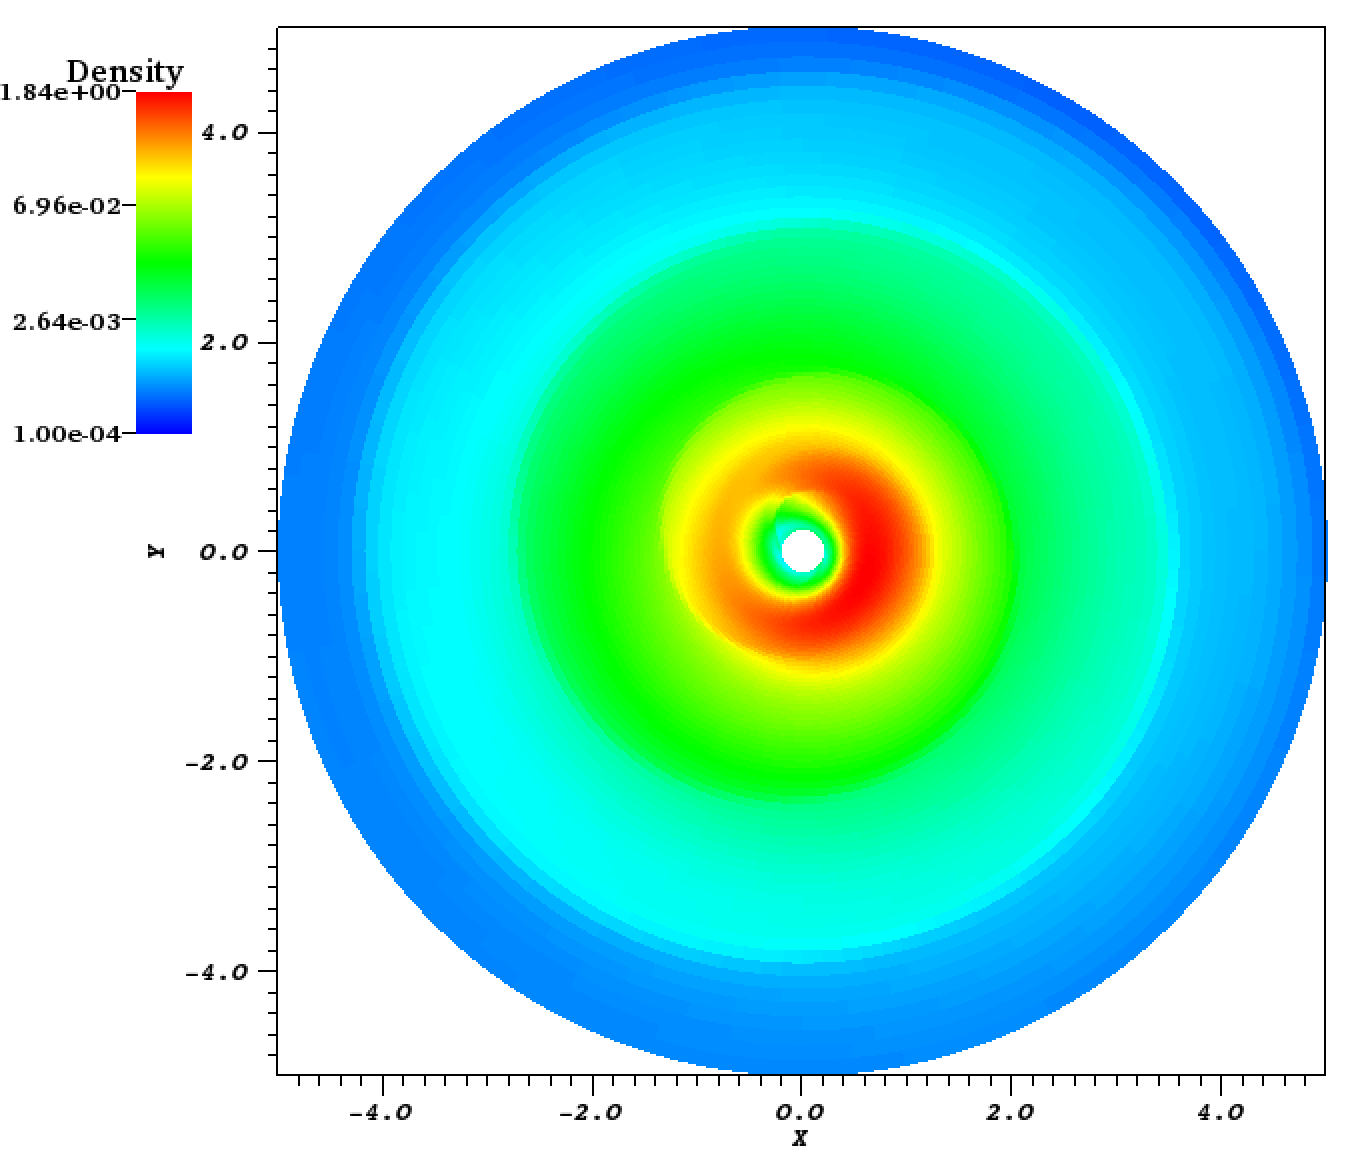
\includegraphics[width=0.45\textwidth]{plots/t32_orbit.png}
\caption{Z-slice of a 3D simulation of the torus showing spiral waves at the nonlinear regime (t=32 orbits). }
\label{t32_orbit}
\end{figure}
\subsubsection{Effects of Distortion Parameter}
\par In Run F,G, we tried using two different distortion parameters that determines the shape of the torus. The value of d=1.1773 is derived from the $r_{in}$ and $r_{out}$ in the A2 slender torus model in \cite{Hawley:1991A}. For qualitative comparison, undistorted torus is smaller with a nearly-circular cross section as d$\rightarrow$1. We find that the behavior of the two runs showed similar evolution, however, all the sequence of events in Run F occurred earlier in Run G than in Run F.
%One possible explanation is that 

\subsubsection{Effects of Logarithmic Gridding}
\par  Increasing the radial dynamic range using logarithmic gridding puts more gas into the computational domain so that the ambient conditions remains realistic for a longer period of time after the instability begins the drive the gas outside of the computational domain. Along with the proper boundary conditions as discussed in Sec~\ref{sec:BC}, we no longer observe low density gas below the $10^{-6}$ density floor. We attempted at different multiplicative factors of logarithmic gridding in Run H, I, J and found that a factor of 1.03 is sufficient for covering the large radial domain. In Run I and J, the large logarithmic factor results in very fine grids near the inner boundary. Since there is high infall velocities due to the pseudo-Newtonian potential, the CFL condition strongly limits the timesteps of the simulation. In the future, \ac{SMR} could be used to increase the resolution near the torus mid-plane region.
\begin{table*}[t]
\centering
    \begin{tabular}{lllllllll}
    \hline
    Run & Grid                   & $\Delta r$ & $R_{in},R_{out}$ & d     & Perturbation & Inner B.C.
(r, $\theta/\phi$) & $t_{run}$ [orbits] & p/d floor \\ \hline
    A & $256\times96\times256$ & 1.03       & 0.2,5.0          & 1.173 & Random,1\%    & 0,corotating                  & ----                 & $10^{-6}$   \\
    B & $64\times64\times64$   & 1          & 0.2,2.5          & 1.173 & Random, 1\%   & 0,0                           & 14.961             & $10^{-8}$   \\
    C & $64\times64\times64$   & 1          & 0.2,2.5          & 1.173 & Random, 1\%   & 0,corotating                  & 31.672             & $10^{-8}$   \\
    D & $64\times64\times64$   & 1          & 0.2,2.5          & 1.173 & Random, 1\%   & outflow,0                     & 8.117              & $10^{-8}$   \\
    E & $64\times64\times64$   & 1          & 0.2,2.5          & 1.173 & Random, 1\%   & outflow,corotating            & 7.003              & $10^{-8}$   \\
    F & $64\times64\times64$   & 1          & 0.2,2.5          & 1.125 & Random, 0.1\% & 0,corotating                  & 156.767            & $10^{-8}$   \\
    G & $64\times64\times64$   & 1          & 0.2,2.5          & 1.173 & Random, 0.1\% & 0,corotating                  & 112.841            & $10^{-8}$   \\
    H & $96\times64\times128$  & 1.03       & 0.2,5.0          & 1.173 & Random, 1\%   & 0,corotating                  & 56.818             & $10^{-6}$   \\
    I & $96\times64\times128$  & 1.05       & 0.2,5.0          & 1.173 & Random, 1\%   & 0,corotating                  & 38.515             & $10^{-6}$   \\
    J & $96\times64\times128$  & 1.09       & 0.2,5.0          & 1.173 & Random, 1\%   & 0,corotating                  & 1.592              & $10^{-6}$   \\
    K & $256\times96\times128$ & 1          & 0.2,2.5          & 1.173 & Random,0.1\%  & 0,corotating                  & 24.048             & $10^{-8}$   \\ 
     L & $96\times64\times128$  & 1.03       & 0.2,5.0          & 1.173 & m=1, 0.1\%   & 0,corotating                  & 1.76               & $10^{-6}$ \\
    M & $96\times64\times128$  & 1.03       & 0.2,5.0          & 1.173 & m=1,0.001\%  & 0,corotating                  & 3.18               & $10^{-6}$ \\ \hline
    \end{tabular}
    \caption{Selected parameters used in simulations.}
 \label{parameters}\end{table*}
 \subsubsection{Effects of Mode Initialization}
\par  We describe two ways of initializing perturbation the simulation to trigger the \ac{PPI}: random initialization and eigenmode initialization. As done in  \cite{Hawley:1991A}, for the random initialization, we added a unique, random number scaled by the amplitude to the gas pressure, which effectively adds enthalpy perturbation to each grid zone. For the eigenmode initialization, we added a perturbation of the form $A_0 sin(m\phi)$ in the $\phi$-component of the momentum, where $A_0$ is the amplitude.
\par We begin by initializing with amplitude of 1\% on the m=1 mode. However, the strong perturbation results in violent, nonlinear evolution within an orbital time. This makes the mode growth analysis difficult as the analytical mode growth derived by \cite{Goldreich:1986A} is based on a linear stability analysis, which does not give accurate prediction in the nonlinear regime after $t_{saturation}$. The 1\% perturbation was acceptable when using the random initialization method because the amplitude of the perturbation does not directly translate into 1\% amplitude for the m=1 mode growth. In the random initialization,  any frequency mode can be possible, so the percentage of the actual amplitude that contributes to one specific mode amplitude is likely to be lower. Therefore, we decreased the amplitude to 0.001\% for the m=1 eigenmode in Run M to conduct the analysis. In both types of initialization, we see strong m=1 mode growth and subsequent higher-order mode growth due to mode coupling.
\section{Magnetorotational Instability}
\par The magnetorotational instability is 




  \subsection{Numerical Methods}
	\subsubsection{Initial Conditions}
	To initialize an azimuthal field, we make use of the three degrees of freedom to set a convenient gauge that enables us to define $A_r = A_\phi = 0$ and $A_\phi = \frac{\rho^2}{\beta_0}$. We define initial conditions using the magnetic scalar potential at cell-corners and then compute $B(r,\theta)$ by $\nabla \times A$, rather than directly defining the initial condition using the face-centered magnetic fields to ensure the $\nabla \cdot \vec{B}=0$ condition is satisfied in the discretized form. Using Stoke theorem to convert the $\vec{B}$ equation into an integral form,
\begin{equation}
\int \vec{B} \cdot d\vec{S}  = \int A\cdot dl 
\end{equation}
we can get the magnetic field by the simple discrete form:
\begin{equation}
\vec{B}=\frac{1}{\Delta S}[A_{\phi,+} l_+ +A_{\phi,-} l_-] .
\end{equation}
	\par $\beta_0$ is a user-defined value for the plasma beta describing the ratio of gas-to-magnetic pressure. To maintain the initial hydrostatic equilibrium of the torus, we need to chose a $\beta$ such that the initial azimuthal magnetic field is weak.
Additionally, $\beta$ is important in determining the number of zones required to resolve MRI per scale height of the system.
\par In the case of \ac{PPI}, there is a strict condition on the rotational velocity profile of constant angular momentum. This is not necessary for \ac{MRI} to take place , in fact a Keplerian disk is okay. 
\subsection{Numerical Results}
\subsubsection{Effects of Resolution}
\par Since the \ac{MRI} is dominated by higher-order modes, as shown in Sec.\ref{mode_growth_mri}, it is crucial that our grids resolve to scales smaller than these in order for to resolve the higher order modes. to generate ---- convergence test with previous results in literature. We employ the 
given in --- to ensure that there are enough resolutoion to .
also demonstrated the robustness of the \app code and its treatment of the ---- magnetic fields . The scale height (H) in our simulation decreases radially outward as $\sqrt{2/r}$. We use the zones-per-scale-height formula in \cite{Hawley:2011A} to compute the minimum zones (N) required in the r direction to resolve the \ac{MRI} and obtained $N_\phi$=223.713. Therefore, we ran a high-resolution simulation with $384\times 256\times 256$ on 768 processors.
conservative 
\section{Comparison of Instabilities}
\subsection{Physical Mechanism}
\paragraph*{\rm{\textbf{\acf{PPI}}\\}}
\par Based on the torus boundaries on the z=0 plane in \citep{Papaloizou:1984A},
\begin{equation}
\tilde{\omega}_\pm  = \frac{\tilde{\omega_0}}{1\mp\sqrt{1-\frac{1}{d}}}
\label{boundary}
\end{equation}
where d is the distortion parameter, we obtained ($\tilde{\omega}_+,\tilde{\omega}_-$) = (1.623, 0.723) for the case of a slender torus. Therefore, the scaled azimuthal wavenumber $\beta$ is related to the wave mode by $\beta = 0.45 m $. The mode growth was computed by linear least square fit on the log-amplitude plot. Since we assume the form of the physical quantity to be $q(t)=q_0 e^{\frac{t}{\tau}}$in the linear stability analysis, we can compute the mode growth by : 
\begin{equation}
\tau = \frac{\Delta t}{log(\frac{x(t)}{x_0})}
\end{equation}
and verified that the values are similar to the previous numerical and analytical studies of mode growth in literature. For the m=1 modes, since the condition $\beta<0.59$ is satisfied, it falls into the class of unstable modes known as the principle branch which has its corotation radius $R_c$ at pressure maximum. \cite{Goldreich:1986A} showed that these can be reasonable approximated with a set of 2D height-integrated equations. The corotation radius ($R_c$) is the radius where the angular speed ($\Omega$)is equal to the pattern speed($\Omega_p$), where the pattern speed is described $Re(\omega)/m$. $R_c$ separates the inner region of the torus with negative action the outer region with positive action.
\par For the principal modes, the instability comes from the coupling between two traveling surface waves launched from the inner and outer edge of the torus. More generally, for higher-order modes, \cite{Narayan:1987A} describes amplification mechanism where the transmitted and reflected wave gets trapped near the evanescent region around $R_c$. With a satisfied phase condition, this amplification mechanism creates a feedback loop that reflects its own output back into the system, thus triggering the unstable mode growth seen in \ac{PPI}. The principal mode is a special case of higher-order modes where the whole torus is the evanescent region, so the only waves that could interact and grow unstable are the traveling surface waves near $\tilde{\omega_\pm}$.
\paragraph*{\rm{\textbf{\acf{MRI}}\\}}
The magnetorotational instability is a local, \ac{MHD}, shearing instability can also be explained from the linear stability analysis of the \ac{MHD} equations, as detailed in the review paper \citep{Balbus:1998A}. The analysis yields a stability criterion for the rotational velocity profile: 
\begin{equation}
(\vec{k}\cdot\vec{u_A})^2> -\frac{d\Omega^2}{d ln R}
\end{equation}
This suggest that there is instability whenever the angular momentum is decreasing radially outward, which is generally true for most astrophysical disks.
\par This criterium makes sense in terms of the mechanical picture as shown in Fig.~\ref{mri_diagram}

\subsection{Mode Growth Analysis}
\par In order to quantify the results of the numerical simulation, we conduct the mode growth analysis and compare our result with the 3D numerical simulations done \cite{Hawley:1991A} and the analytical growth rates given by \cite{Goldreich:1986A}. To motivate the analysis of the eigenmodes, we first consider the physical mechanisms that give rise to \ac{PPI} summarized in \cite{Narayan:1989A}.
\par The \ac{PPI} give rise to unstable was modes that grows exponentially in time. We quantify the mode amplitudes by conducting a Fourier decomposition in the $\phi$ direction. The number of zones in the $\phi$ direction was chosen for this purpose to powers of two in order to speed up the \ac{FFT} algorithm used to extract the modes. 
\par We use a Python package \texttt{h5py} to read in the simulation data stored in HDF5 format per timestep. For every meshblock the datafile, we first compute the mass enclosed per cell in each $\Delta\phi$ slice by :
\begin{equation}
\frac{\mbox{\large M}_{\mbox{enclosed}}}{\Delta\phi} = \rho\Delta V_{\mbox{cell}} = \rho r^2 sin\theta \Delta r \Delta\theta
\end{equation}
\begin{equation}
D(\phi) = \sum_r \sum_\theta \rho \frac{\Delta V_{\mbox{cell}}}{\Delta\phi}
\end{equation}
Due to the z-ordering in the \app\textit{'s} internal data structure, we use the the logical locations stored in each meshblock and sum over all the mass in a particular $r-\theta$ slice. This yields a 1D-array of length 128 containing the integrated mass per slice, $D(\phi)$. Then by Fourier decomposing the wave into 128 bins, we compute the magnitude by $|A|=\sqrt{\tilde{A}\cdot \tilde{A}^*}$. Fig.~\ref{m1init1E-5} and ~\ref{randinit1percent} shows the mode growth of the m=1-5 modes. 
\begin{figure}
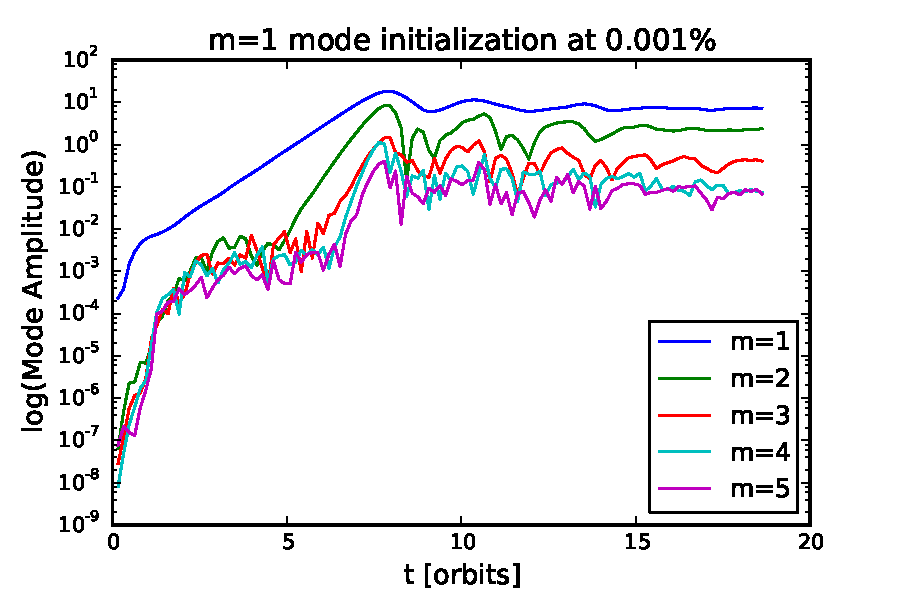
\includegraphics[width=0.45\textwidth]{plots/m1init1E-5.pdf}
\caption{Mode growth of the m=1-5 initialized with m=1 mode at 0.001\%.}
\label{m1init1E-5}
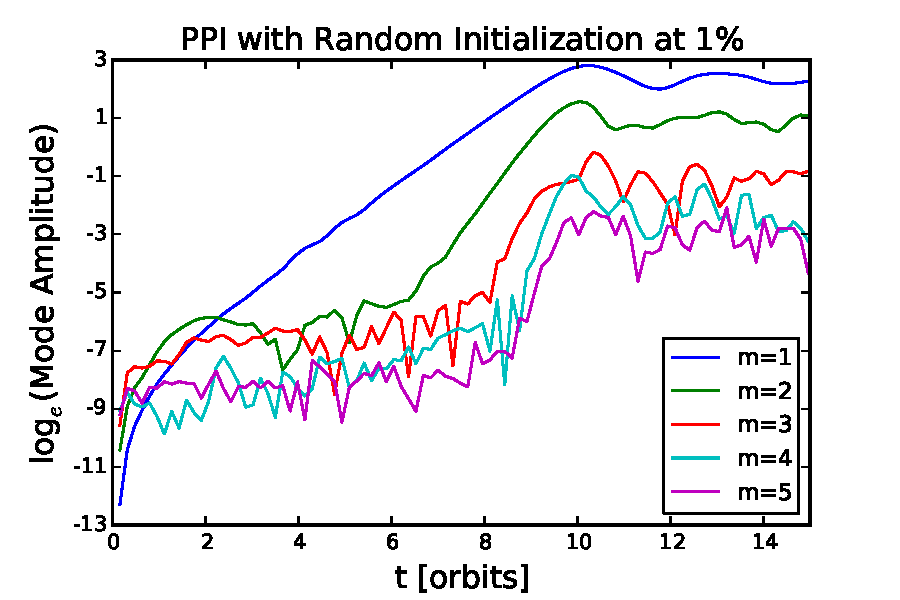
\includegraphics[width=0.45\textwidth]{plots/randinit1percent.pdf}
\caption{Mode growth of the m=1-5 with random initialization at 1\%.}
\label{randinit1percent}
\end{figure}
Table~\ref{mode_growth} summarizes the mode growth comparison with \cite{Hawley:1990A} for the random and eigenmode (m=1) initialization.
\begin{table}
\centering
    \begin{tabular}{|l|l|l|}
    \hline
    ~   & Random Initialization & Eigenmode Initialization \\ \hline
    m=1 & 0.8679\quad0.855      & 0.2667\quad0.2621        \\
    m=2 & 0.4701\quad0.211      & 0.5505\quad0.5100        \\
    m=3 & 0.3756\quad0.254      & 0.6828\quad0.6820        \\ \hline
    \end{tabular}
    \caption{Left-flushed values are the mode growth in Run J, M respectively; right-flushed values are mode growth in \cite{Hawley:1991A}.}
    \label{mode_growth}
\end{table}
\subsection{Mass Accretion History}
We compute the accretion onto the inner boundary by computing the radial component of the momentum in the innermost cell.
\begin{equation}
\frac{dM}{dt}=\sum_{j,k} \rho v_r \Delta S_{i,j_{\pm},k}
\end{equation}
As shown in Fig.\ref{mass_accretion}, the mass accretion rate history in our simulation qualitatively agrees with the accretion rate history in \cite{Jiang:2014A}. In addition, we find that the mass accretion rate in the \ac{MRI} case is much stronger than that of the \ac{PPI}.
\begin{figure}[h]
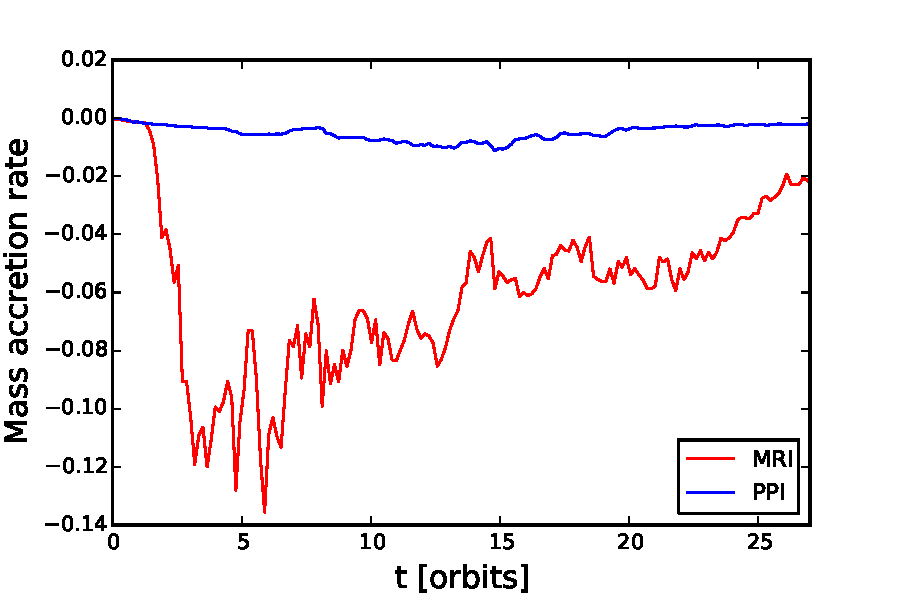
\includegraphics[width=0.45\textwidth]{plots/mass_accretion.pdf}
\caption{The mass accretion rate that results from the instabilities.}
\label{mass_accretion}
\end{figure}
\section{Conclusion}
\par In this study, we use ------ using the \app code to investigate the \acf{MRI} and \acf{PPI}.

\par The 
From the mass accretion history of the -----, which explains the recent interest in studying the \ac{MRI}.
\acknowledgments
\section*{Acknowledgments}
I thank Kengo Tomida and Jim Stone for mentoring and support in this summer project. This research used resources of the National Energy Research Scientific Computing Center, a DOE Office of Science User Facility supported by the Office of Science of the U.S. Department of Energy under Contract No. DE-AC02-05CH11231.
\bibliography{bibdatabase}
\end{document}

